\documentclass{"../../res/univ-projet"}
\usepackage[utf8]{inputenc}
\usepackage{array}
\usepackage[T1]{fontenc}
\usepackage[francais]{babel}

\logo{../../res/logo_univ.png}
\title{Spécification Technique des Besoins}
\author{Maxime \bsc{Michotte}, Benjamin \bsc{Zigh}}
\projet{M1SSI}
\projdesc{Projet de génération d'OTP}
\filiere{M1SSI}
\version{2.0}
\relecteur{Damien \bsc{Picard}}
\signataire{Magali \bsc{Bardet}}
\date{Janvier 2014}

\histentry{3.0}{30/01/14}{Nouvelle version de base}
\histentry{2.0}{16/01/2014}{Version pour la revue de lancement.}
\histentry{1.3}{15/12/2013}{Ajout des modifications demandées par le client}
\histentry{1.2}{04/12/2013}{Ajout des exigences correspondant au CdR}
\histentry{1.1}{28/11/2013}{Ajout terminologie et modification schémas}
\histentry{1.0}{15/11/2013}{Version initiale.}


\begin{document}
\maketitle
%-------------------------------------------------------------------------------
\section{Objet}
Ce document définit les exigences de l'étude et l'implémentation des systèmes d'authentification 
utilisant des mots de passe jetables ainsi que leurs domaines de fonctionnement.

    \subsection{Besoins opérationnels} 
        \begin{itemize}
            \item Garantir une authentification forte.
            \item État de l'art sur les systèmes existants.
            \item Objectif : mise en production.
        \end{itemize}
    \subsection{Objectifs techniques}
    \begin{itemize}	
            \item Implémentation des solutions retenues sur un ou plusieurs supports.
    \end{itemize}
    \subsection{Contraintes et recommandations} 
        \begin{itemize}
            \item Respecter les spécifications de base et les normes RFC.
            \item Montrer que le système produit est sûr.
            \item Choisir une implémentation adaptée en fonction des besoins et de l'état de l'art établi.
        \end{itemize}
    \subsection{Résultats attendus} 
        \begin{itemize}
            \item Système sûr et fonctionnel.
            \item État de l'art le plus exhaustif possible.
            \item Implémentation sur Carte à puces et/ou Android.
        \end{itemize}
        
\newpage
%-------------------------------------------------------------------------------
\section{Documents applicables et de référence}

\begin{tabular}{p{1,5cm}>{\raggedright\arraybackslash}p{13cm}}
{[sujet]} & {Expression du besoin client: Étude et implémentations des systèmes d'authentification utilisant des mots de passe jetables.}
\tabularnewline
\\
{[goo]} & {Google Authenticator \href{https://code.google.com/p/google-authenticator/}{https://code.google.com/p/google-authenticator/}.}
\tabularnewline
\\
{[ANS10]} & {ANSSI. Référentiel général de sécurité. \href{http://www.ssi.gouv.fr/fr/reglementation-ssi/referentiel-general-de-securite}{http://www.ssi.gouv.fr/fr/reglementation-ssi/referentiel-general-de-securite}, 2010.}
\tabularnewline
\\
{[MvOV97]} & {Alfred J. Menezes, Paul C. van Oorschot, and Scott A. Vanstone. Handbook of applied cryptography. CRC Press Series on Discrete Mathematics and its Applications. CRC Press, Boca Raton, FL, 1997. With a foreword by Ronald L.Rivest.}
\tabularnewline
\\
{[RFC98]} & {A One-Time Password System. \href{http://tools.ietf.org/html/rfc2289}{http://tools.ietf.org/html/rfc2289}, 1998.}
\tabularnewline
\\
{[RFC05]} & {HOTP:An HMAC-Based One-Time Password Algorithm \href{http://tools.ietf.org/html/rfc4226}{http://tools.ietf.org/html/rfc4226}, 2005.}
\tabularnewline
\\
{[RFC06]} & {Generic Message Exchange Authentication for the Securer Shell Protocol (SSH).\href{http://tools.ietf.org/html/rfc4256}{http://tools.ietf.org/html/rfc4256}, 2006.}
\tabularnewline
\\
{[RFC07]} & {The EAP Protected One-Time Password Protocol (EAP-POTP). \href{http://tools.ietf.org/html/rfc4793}{http://tools.ietf.org/html/rfc4793}, 2007.}
\tabularnewline
\\
{[RFC11]} & {TOTP: Time-Based One-Time Password Algorithm \href{http://tools.ietf.org/html/rfc6238}{http://tools.ietf.org/html/rfc6238}, 2011.}
\tabularnewline
\\
{[goo]} & {Google Authenticator \href{https://code.google.com/p/google-authenticator/}{https://code.google.com/p/google-authenticator/}.}
\tabularnewline
\\
\end{tabular}

%-------------------------------------------------------------------------------
\section{Exigences fonctionnelles}
\begin{tabular}{|c|l|l|c|}
    \hline
    \rowcolor{gray}
    \textcolor{white}{Id} & \textcolor{white}{Intitulé} & \textcolor{white}{Acteur(s)} & \textcolor{white}{Priorité}\\
    \hline
    EF\_01 & État de l'art & Équipe & Indispensable\\
    \hline
    EF\_02 & Association serveur-client-token & Utilisateur & Indispensable\\
    \hline
    EF\_03 & Génération de l'OTP par le token & Utilisateur & Indispensable\\
    \hline
    EF\_04 & Authentification & Utilisateur & Indispensable\\
    \hline
    EF\_05 & Re-synchronisation & Utilisateur & Indispensable\\
    \hline
\end{tabular}\

\begin{figure}[h]
  \centering
  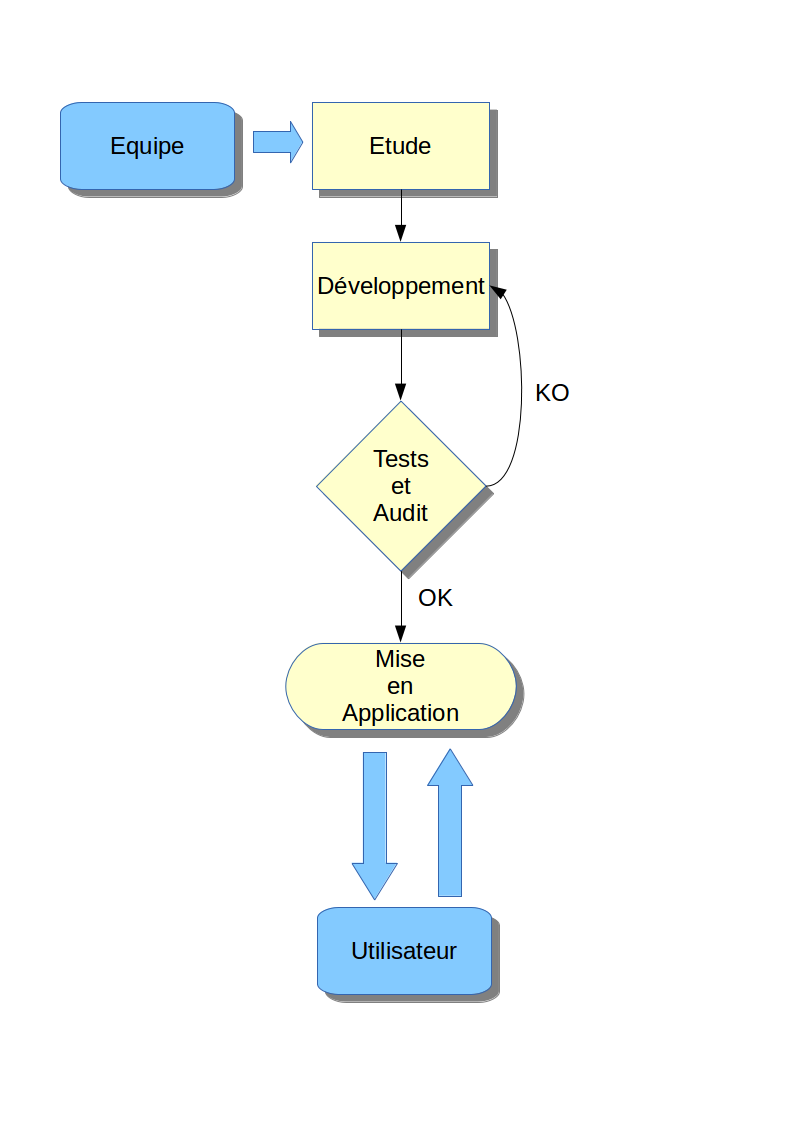
\includegraphics[scale=0.5]{../graphics/diagramme1.png}
  \caption{Schéma Macroscopique du Projet}
  \setlength{\parindent}{1cm}
  \begin{flushleft}
  Nous (l'équipe) commencerons par une étude de la \href{http://tools.ietf.org/html/rfc2289}{RFC2289} et toutes les RFC basées sur celle-ci
  soit, \href{http://tools.ietf.org/html/rfc4226}{RFC4226}, \href{http://tools.ietf.org/html/rfc4256}{RFC4256}, 
  \href{http://tools.ietf.org/html/rfc4793}{RFC4793}, \href{http://tools.ietf.org/html/rfc6238}{RFC6238} afin de fournir un état de l'art le plus exhaustif possible. Une fois celui-ci terminé nous passerons à
  l'implémentation des meilleurs protocoles retenus. Enfin, pour vérifier notre production,
  un audit sera organisé ainsi qu'une batterie de tests afin de corriger les erreurs de développement pour nous mener \`{a} 
  une mise en application. 
  \end{flushleft}
\end{figure}

\clearpage

\fiche{Association serveur-client-token}{Utilisateur}{Le serveur communique au Token un secret}{Il existe une communication client-serveur}{Bouton utilisateur}{Association réussie}{../graphics/association.jpg}{Impossible d'associer le token au serveur}

\vspace{0.5cm}


L'association serveur-client-token décrit l'intervention de l'utilisateur voulant associer son token au serveur, c'est un processus d'initialisation ou le client
demande à travers son application un secret au serveur. Le serveur génère le secret et le retourne au client. L'utilisateur entre alors son secret dans le token.

\vspace{1cm}


\fiche{Génération de l'OTP par le token}{Utilisateur}{L'utilisateur demande au token un nouvel OTP qui lui est retourné}{Le token est lié au serveur}{L'utilisateur demande un OTP}{OTP généré}{../graphics/generation.jpg}{Null}

\vspace{0.5cm}


Ce protocole décrit la Génération de l'OTP par le token grâce à une demande de l'utilisateur.
\\
\fiche{Authentification}{Utilisateur}{L'utilisateur tente de s'authentifier sur le serveur}{L'utilisateur possède un OTP}{L'utilisateur donne le mot de passe au serveur}{Utilisateur authentifié ou rejeté}{../graphics/authentification.jpg}{Crash du serveur}

\vspace{0.5cm}


L'Authentification permet de valider la légitimité d'un utilisateur; ce protocole décrit une demande d'authentification auprès du serveur pour cela l'utilisateur
entre un mot de passe à travers le client. Le client se charge alors de se connecter au serveur afin de procéder à un test de validation du mot de passe; si celui-ci
est accepté alors le client est authentifié sinon il peut réessayer un mot de passe, au bout de n tentatives celui-ci est rejeté.
\\
\fiche{Re-Synchronisation}{Utilisateur}{Mise en accord du token et du serveur}{Il existe une connexion entre le token et le serveur}
{Perte de la synchronisation}{Synchronisation retrouvé}{../graphics/resynchronisation.jpg}{Ne peut pas re-synchroniser}

\vspace{0.5cm}

Lors d'une demande d'authentification au serveur, soit le client est identifié, soit l'identification est un échec et dans ce cas
le serveur tente une resynchronisation.
\clearpage
\newpage
%-------------------------------------------------------------------------------
\section{Exigences opérationnelles}
\begin{tabular}{|c|l|c|}
    \hline
    \rowcolor{gray}
    \textcolor{white}{Id} & \textcolor{white}{Intitulé} & \textcolor{white}{Priorité}\\
    \hline
    EP\_01 & Le Token renvoie un OTP & Indispensable\\
    \hline
    EP\_02 & L'OTP est utilisable 1 seule fois & Indispensable\\
    \hline
    EP\_03 & L'OTP est non prévisible (OTP qui ne peut être déduit des anciens générés) & Indispensable\\
    \hline
    EP\_04 & Résistant à une attaque exhaustive & Indispensable\\
    \hline
    EP\_05 & Résistant aux attaques par rejeu & Indispensable\\
    EP\_06 & Respect des RFC (RFC2289, RFC4226, RFC4256, RFC4793, RFC6238) & Indispensable\\
    \hline
    \hline
    
    
\end{tabular}

%-------------------------------------------------------------------------------
\section{Exigences d'interface}
\begin{tabular}{|c|l|c|}
    \hline
    \rowcolor{gray}
    \textcolor{white}{Id} & \textcolor{white}{Intitulé} & \textcolor{white}{Priorité}\\
    \hline
    EI\_01 & UNIX(Client/Serveur/Token) & Indispensable\\
    \hline
    EI\_02 & Android(Token) & Indispensable\\
    \hline
    EI\_03 & Java Card (Token) & Facultatif\\
    \hline
\end{tabular}
\vspace{0.5cm}
\begin{description}
 \item[Unix] Unix désigne pour notre cas un système GNU/Linux et afin de permettre une plus grande compatibilité
 nous acceptons les kernels de version 3.x ainsi que glibc supérieur à la version 2.15.
 \item[Android] Android désigne pour notre cas toutes les terminaux mobiles tournant sous le système d'exploitation Android en version 2.3.x et 4.x.
\end{description}

%-------------------------------------------------------------------------------
\section{Exigences de qualité}
\begin{tabular}{|p{0.1\textwidth}|p{0.7\textwidth}|p{0.15\textwidth}|}
    \hline
    \rowcolor{gray}
    \textcolor{white}{Id} & \textcolor{white}{Intitulé} & \textcolor{white}{Priorité}\\
    \hline
    EQ\_01 & Génération de mots de passe inférieur à 1 seconde (sur un processeur cadencé à 700MHz) & Indispensable\\
    \hline
    EQ\_02 & Temps de réponse serveur (temps < 1 sec + 2 * tps communication) & Indispensable\\
    \hline
    EQ\_03 & Le serveur supporte au moins 100 000 demandes de vérification simultanées & Important\\
    \hline
    EQ\_04 & La vérification est cohérente & Indispensable\\
    \hline
    EQ\_05 & La génération utilise au plus 10 Ko de mémoire & Important\\
    \hline
    EQ\_06 & état de l'art exhaustif, au moins trois protocoles OTP étudiés & Indispensable\\
    \hline
\end{tabular}
%-------------------------------------------------------------------------------
\end{document}
